\chapter{Deep Learning}

\section{Introducción}
% The basic unit is the so-called neuron
% I A Linear Discriminant Function (LDF)
% I With an activation function

\begin{paracol}{2}
   La unidad basica es el llamado \textbf{neuron}, que implementa una \textit{Función Discriminante Lineal} (\textsc{LDF}) con una función de activación. Un neurón recibe múltiples entradas, aplica pesos a estas entradas, suma los resultados y pasa esta suma a través de una función de activación para producir una salida.
   
   \switchcolumn

   \begin{figure}[htbp]
      \centering
      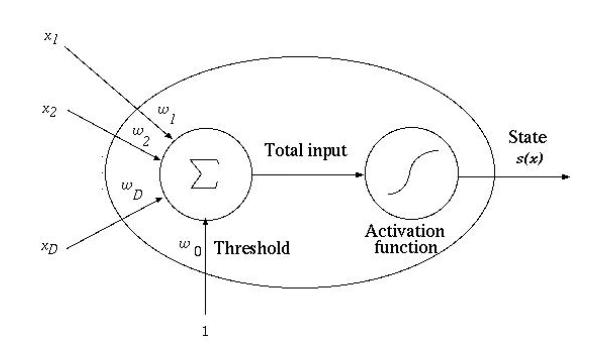
\includegraphics{images/08/neuron.png}
      \caption{Neuron}
      \label{fig:08/neuron}
   \end{figure}

\end{paracol}

Matemáticamente, un neurón se puede representar como:

\[ y = f\left(\sum_{i=1}^{n} w_i x_i + b\right) \]

Donde:
\begin{itemize}
   \item $x_i$ son las entradas
   \item $w_i$ son los pesos
   \item $b$ es el sesgo (bias)
   \item $f$ es la función de activación
\end{itemize}

Neurones pueden ser combinados en \textsc{capas} (\textit{layers}): lineal layers, convolutional layers, recurrent layers, etc.
Capas pueden ser combinados en redes neuronales (\textit{neural networks}).

\begin{figure}[htbp]
   \centering
   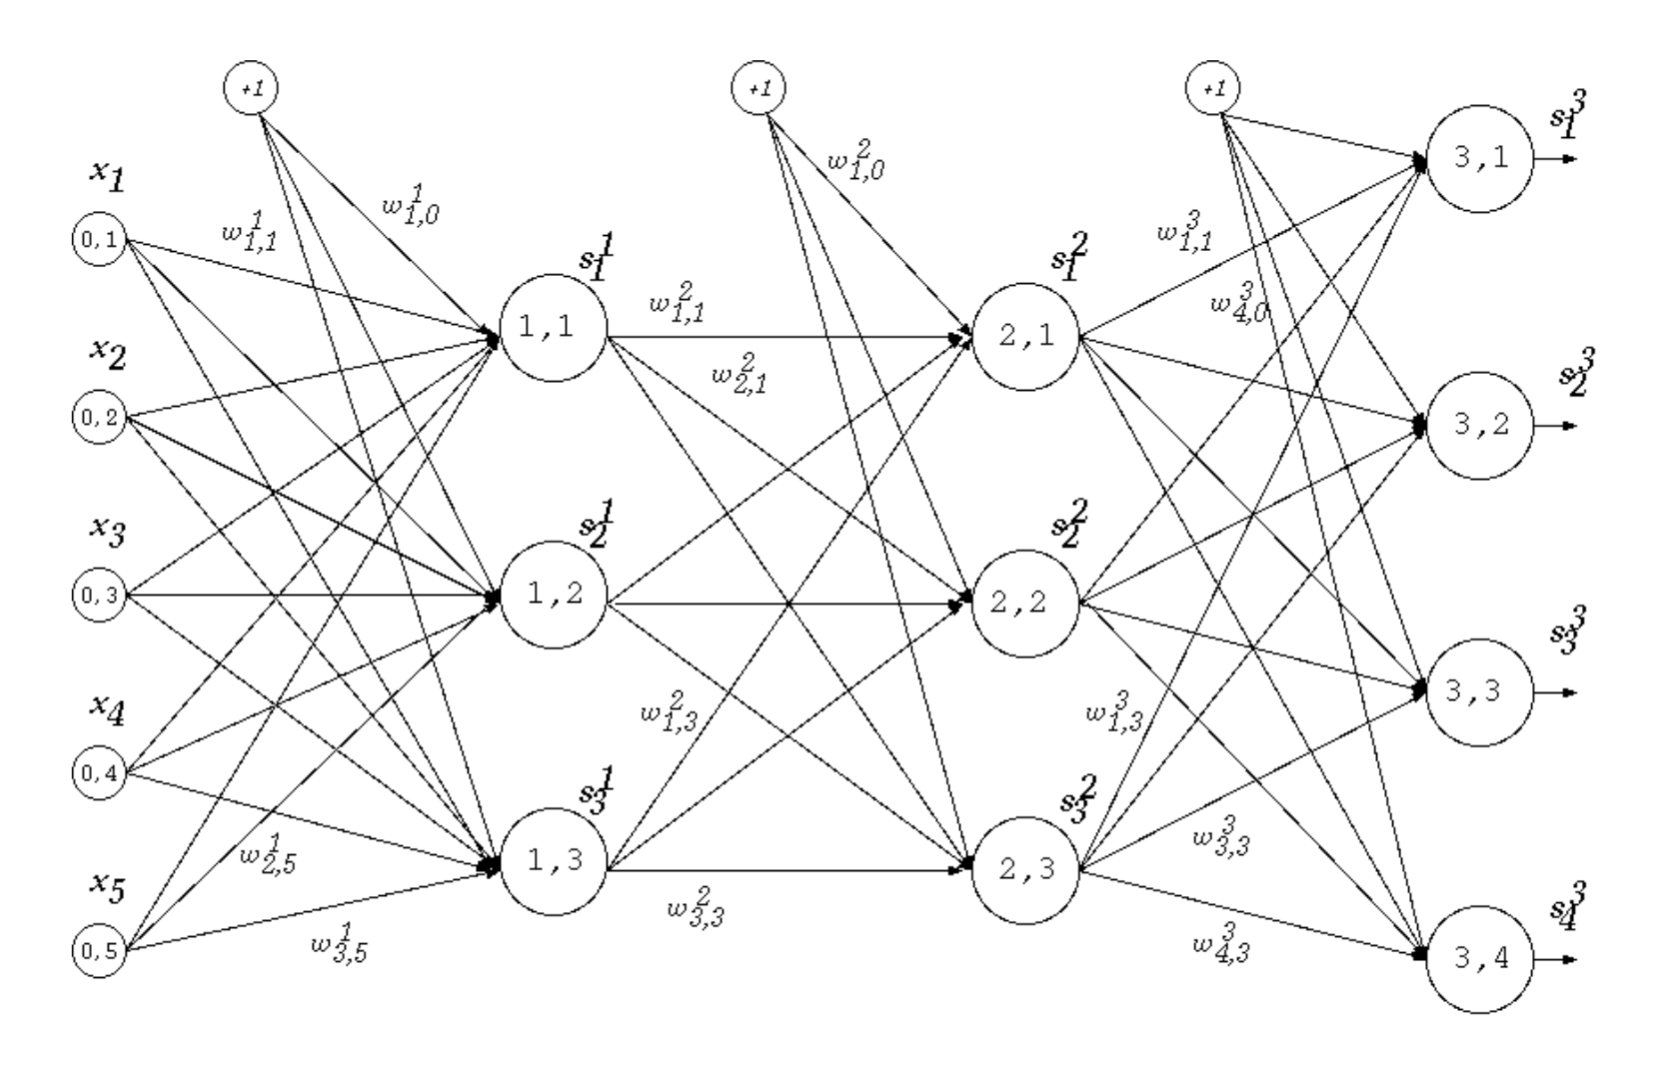
\includegraphics{images/08/layers1.png}
   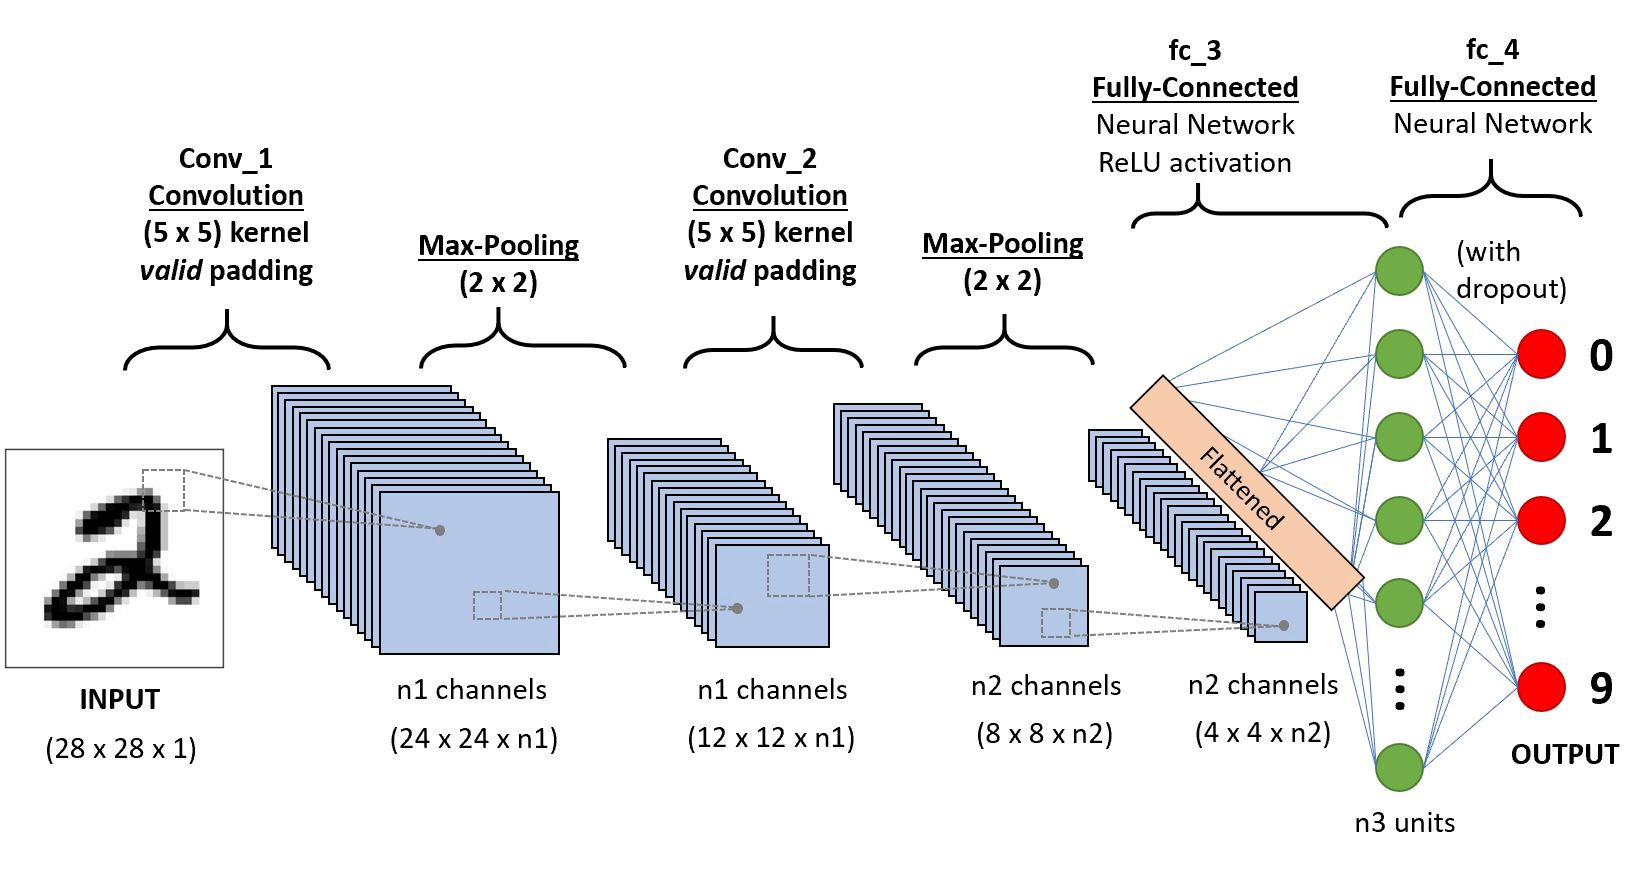
\includegraphics{images/08/layers2.jpeg}
   \caption{Capas y redes neuronales}
   \label{fig:08/layers}
\end{figure}

\section{Linear Discriminant Function and Perceptron}

A classifier $G$ in $C$ classes can be defined by $C$ discriminant functions $g_c$.\\
Classification rule $(\vec{x} \in \mathbb{R}^D ): \hat{c} = G(\vec{x}) = arg max_{c=1},...,C g_c (\vec{x})$

\begin{figure}[htbp]
   \centering
   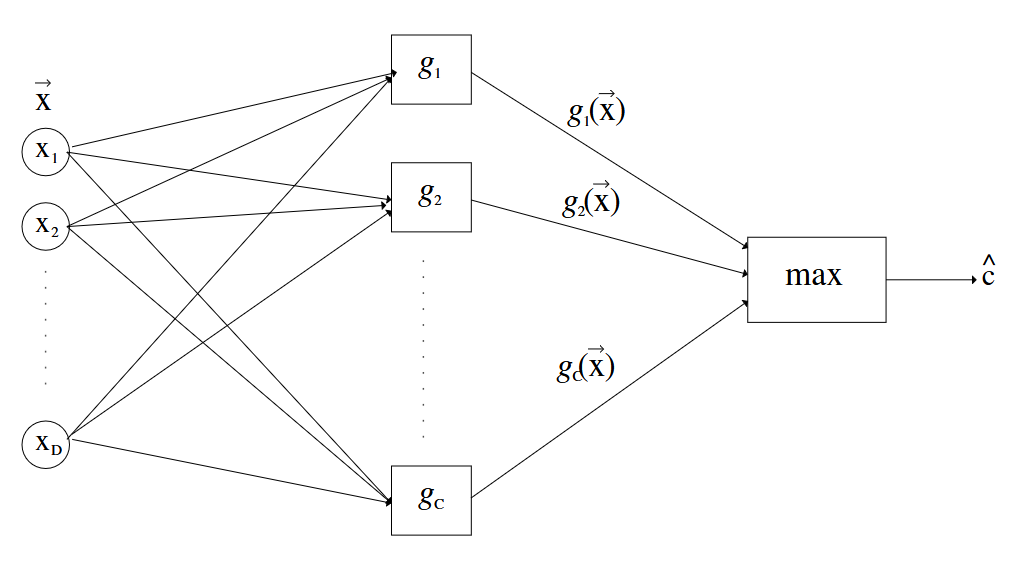
\includegraphics{images/08/discriminant.png}
   \caption{Discriminant function Graph}
   \label{fig:08/discriminant}
\end{figure}

When $g_c$ are linear functions, they are called \textbf{Linear Discriminant Functions} (\textsc{LDF})
\[
   g(\vec{x}) = w0 + \sum^D_{i=1}\vec{w_i} \vec{x_i} = w0 + \vec{w^t} \vec{x}
   \]
$\vec{w}$ is the weights vector, w0 is the bias term
In homogeneus notation: $w = (w0, \vec{w^t} )t , x = (1, \vec{x^t} )t$
\[g(\vec{x}) = w^t x\]
G is a linear classifier when all $g_c$ are linear functions, with parameters $w_c$
Given a training dataset of samples in $\mathbb{R}^D$, $w_c$ can be estimated by \ul{using the
\textbf{Perceptron} algorithm}

\begin{figure}[htbp]
   \centering
   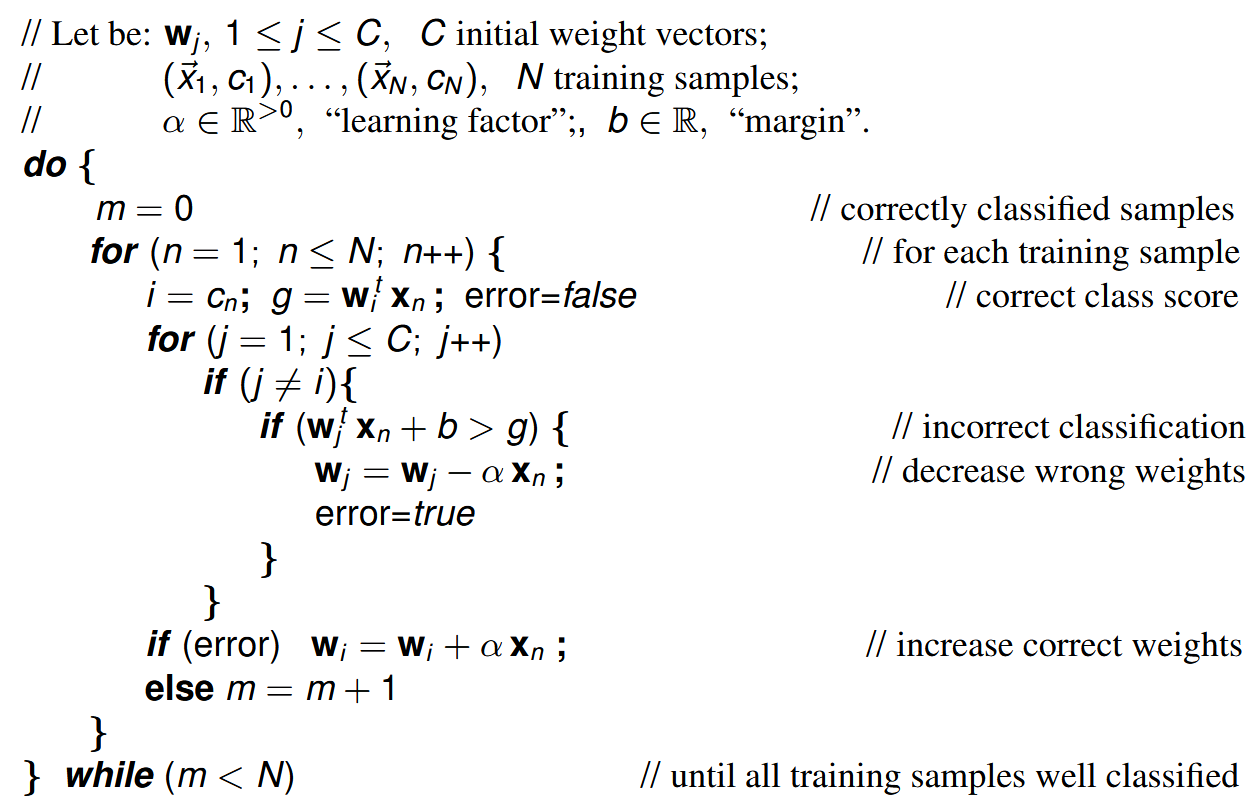
\includegraphics{images/08/perceptron.png}
   \caption{Perceptron algorithm}
   \label{fig:08/perceptron}
\end{figure}

\begin{algorithm}
   \caption{Perceptron algorithm}\label{euclid}
   \begin{algorithmic}[1]
      \State Perceptron algorithm
      \State // Let be: $w_j , 1 \leq j \leq C, C$ initial weight vectors;
      \State // $(\vec{x_1}, c_1), \dots , (\vec{x_N} , c_N ), N  $ training samples;
      \State // $\alpha \in \mathbb{R}>0, ``learning factor'', b \in \mathbb{R}$, ``margin''.
      % \Procedure{MyProcedure}{}
      % \EndProcedure
\end{algorithmic}
\end{algorithm}

The main limitation is that LDF provide linear frontiers only linearly separable classes
can be properly separated
Using margin b allows for a non-optimal solution
Combining several LDF in cascade does not solve the problem
Result is still an LDF
Solution: use of Activation Functions → Logistic LDF (neuron)